\section{Teoremas de Fubini y Tonelli}

\subsection{Teorema de Tonelli}
Notación:
\[
    \mathbb{R}^{n+k} = \mathbb{R}^n \times \mathbb{R}^k \qquad (x, y)
    = (x_1, \dots, x_n, y_1, \dots, y_k) \in \mathbb{R}^{n+k}
\]
Sea $f: \mathbb{R}^{n+k} \to [-\infty, +\infty]$, entonces denotamos las
funciones:
\[
    \begin{cases}
        f_{x}: \mathbb{R}^k \to [-\infty,+ \infty] \quad \text{con} \quad f_{x}(y) = f(x, y) \quad \forall y \in \mathbb{R}^k \\
        f_{y}: \mathbb{R}^n \to [-\infty,+ \infty] \quad \text{con} \quad f_{y}(x) = f(x, y) \quad \forall x \in \mathbb{R}^n
    \end{cases}
\]

\begin{teorema}[Teorema de Tonelli]
    Sea $f : \mathbb{R}^{n+k} \to [0, +\infty]$ medible. Entonces:
    \vspace{-0.5em}
    \begin{enumerate}
        \item Para casi todo $x \in \mathbb{R}^n$, la función $f_{x} : \mathbb{R}^k \to [0,
                      +\infty]$ es medible en $\mathbb{R}^k$
        \item La función $F: \mathbb{R}^n \to [0, +\infty]$ tal que $F(x) =
                  \int_{\mathbb{R}^k}f_x = \int_{\R^k} f(x,y)dy$ definida en casi todo punto de
              $\R^n$ es medible en $\mathbb{R}^n$
        \item $\int_{\mathbb{R}^{n+k}}f = \int_{\mathbb{R}^n}F = \int_{\mathbb{R}^n}(\int_{\mathbb{R}^k}f_x) = \int_{\mathbb{R}^n}(\int_{\mathbb{R}^k}f(x,y)dy)dx = \int_{\mathbb{R}^{n+k}}f(x,y)dxdy$
    \end{enumerate}
    Además, de forma análoga se tiene que:
    \vspace{-0.5em}
    \begin{enumerate}
        \item Para casi todo $y \in \mathbb{R}^k$, la función $f_{y} : \mathbb{R}^n \to [0,
                      +\infty]$ es medible en $\mathbb{R}^n$.
        \item La función $G: \mathbb{R}^k \to [0, +\infty]$ tal que $G(y) =
                  \int_{\mathbb{R}^n}f_y = \int_{\R^n} f(x,y)dx$ definida en casi todo punto de
              $\R^k$ es medible en $\mathbb{R}^k$.
        \item $\int_{\mathbb{R}^{n+k}}f = \int_{\mathbb{R}^k}G = \int_{\mathbb{R}^k}(\int_{\mathbb{R}^n}f_y) = \int_{\mathbb{R}^k}(\int_{\mathbb{R}^n}f(x,y)dx)dy = \int_{\mathbb{R}^{n+k}}f(x,y)dydx$
    \end{enumerate}
\end{teorema}

\begin{observación}
Los siguientes lemas son previos y necesarios para la demostracion del Teorema de Tonelli.
\end{observación}

\begin{lema}
    Sean $f,g$ que satisfacen el Teorema de Tonelli y $a, b \geq 0 \implies af + bg$ también satisfacen el Teorema de Tonelli\label{lema1Tonelli}
\end{lema}

\begin{proof}
    \leavevmode
    \begin{enumerate}
        \item $\forall x \in \mathbb{R}^n, \ (af + bg)_x = a(f_x) + b(g_x)$ es medible en $\mathbb{R}^k$.
        \item $H(x) = \int_{\mathbb{R}^k}(af + bg)_x = \int_{\mathbb{R}^k}a(f_x) + b(g_x) = \int_{\mathbb{R}^k}a(f_x) + \int_{\mathbb{R}^k}b(g_x)$ es medible en $\mathbb{R}^n$.
        \item $\int_{\mathbb{R}^{n}}(af +bg)_x = a\int_{\mathbb{R}^{n+k}}f_x + b \int_{\mathbb{R}^{n+k}}g_x$
    \end{enumerate}
\end{proof}

\begin{lema}
    Sea $(f_j)_{j\int\mathbb{N}}$ sucesion de funciones que satisfacen el Teorema de Tonelli y $f_j \uparrow f$ en $\mathbb{R}^{n+k}$ puntualmente $\implies$ f satisface el Teorema de Tonelli.\label{lema2Tonelli}
\end{lema}
\begin{proof}
    \leavevmode
    \begin{enumerate}
        \item Para casi todo $x \in \mathbb{R}^{n}$ se tiene que $f_j(x, \cdot) = (f_j)_x
                  \uparrow f(x, \cdot) = f_x$
        \item $F_j(x) = \int_{\mathbb{R}^k}(f_j)_x \uparrow \int_{\mathbb{R}^k}f_x = F(x)$ luego $F$ es medible por el Teorema de la Convergencia Monótona.
        \item Nuevamente por el Teorema de la Convergencia aplicado a la sucesión de (2)
              $F_j(x) \uparrow F(x)$ tenemos que $\int_{\mathbb{R}^{n+k}}f = \lim_{j \to
                      \infty} \int_{\R^{n+k}} f_j = \lim_{j \to \infty}\int_{\mathbb{R}^n}F_j =
                  \int_{\mathbb{R}^n}F = \int_{\mathbb{R}^n}(\int_{\mathbb{R}^k}f(x,y) \,dy)\,dx$
    \end{enumerate}
\end{proof}
\begin{observación}
El siguiente lema es una versión del lema anterior en el que se usa el teorema de la convergencia dominada en lugar del de la convergencia monótona.
\end{observación}

\begin{lema}
    Sea $(f_j)_{j\int\mathbb{N}}$ sucesion de funciones que satisfacen el Teorema de Tonelli. Supongamos que $(f_j)\to f$ puntualmente en $\mathbb{R}^{n+k}$ y $\exists g: \mathbb{R}^{n+k} \to [0, +\infty]$ integrable, que satisface el Teorema de Tonelli y tal que $ 0 \leq f_j \leq g \quad \forall j \in \mathbb{N}$. Entonces, $f$ satisface el Teorema de Tonelli.\label{lema3Tonelli}
\end{lema}
\begin{proof}
    \leavevmode
    \begin{enumerate}
        \item $(f_j)_x \to f_x$ medible
        \item $\int_{\mathbb{R}^{n+k}}g = \int_{\mathbb{R}^n}(\int_{\mathbb{R}^k}g_x) < +\infty$ luego $G(x) = \int_{\mathbb{R}^k}g_x < +\infty$ para casi todo $x \in \mathbb{R}^n$
              Además, tenemos que $0 \leq (f_j)_x \leq g_x$ integrable, por lo que podemos usar el Teorema de la Convergencia Dominada $\implies$
              $F_j(x) = \int_{\mathbb{R}^k}(f_j)_x \to F(x) = \int_{\mathbb{R}^k}f_x$
        \item De nuevo por el Teorema de la Convergencia Dominada $\int_{\mathbb{R}^n}F =
                  \lim_{j \to \infty}\int_{\mathbb{R}^n}F_j = \lim_{j \to
                      \infty}\int_{\mathbb{R}^{n+k}}f_j = \int_{\mathbb{R}^{n+k}}f$
    \end{enumerate}
\end{proof}

\begin{proof}[Demostración del Teorema de Tonelli:]
\leavevmode
\begin{enumerate}
\item Primero veamos el caso en el que \( f \) es la función
indicatriz/característica de un cubo semiabierto.
\begin{enumerate}
\item Supongamos que \( f = \chi_Q \) donde \( Q \) es un cubo semiabierto en \(
\mathbb{R}^{n+k} = \mathbb{R}^n \times \mathbb{R}^k \), con \( Q = A \times B
\) donde \( A \subset \mathbb{R}^n \) y \( B \subset \mathbb{R}^k \).

\begin{observación}
$(\chi_E)_x = \chi_{E_x}  \iff (\chi_E)_x(y) = \chi_E(x, y) = \begin{cases} 1 & (x, y) \in E \\ 0 & (x, y) \notin E \end{cases} = \chi_{E_x}(y)$
\end{observación}

Definiendo:

$$
    f_x = (\chi_Q)_x(y) = \begin{cases}
        \chi_B(y), & x \in A    \\
        0,         & x \notin A
    \end{cases}
$$

Se concluye que \( f_x \) es medible.

\item Definimos la función:

$$
    F(x) = \int_{\mathbb{R}^k} (\chi_Q)_x \, dy = \begin{cases}
        \int_{\mathbb{R}^k} \chi_B \, dy, & x \in A    \\
        0,                                & x \notin A
    \end{cases} =
    \begin{cases}
        m_k(B), & x \in A    \\
        0,      & x \notin A
    \end{cases}
$$

Como resultado, \( F(x) = m_k(B) \cdot \chi_A(x) \) es medible.

\item $$\int_{\mathbb{R}^{n+k}}\chi_Q = m_{n+k}(Q) = m_n(A) \cdot m_k(B) = \int_{\mathbb{R}^n}m_k(B) \cdot \chi_A(x) = \int_{\mathbb{R}^n}F(x)$$

\end{enumerate}

\item Ahora supongamos que \( f \) es la función indicatriz de un conjunto abierto \(
G \subset \mathbb{R}^{n+k} \).

Dado que \( G \) es abierto, se puede escribir como la unión numerable de cubos
semiabiertos disjuntos:

$$
    G = \bigcup_{j \in \mathbb{N}} Q_j
$$

Definiendo \( G_j = \bigcup_{i=1}^{j} Q_i \), se tiene que:

$$
    (G_j) \uparrow G, \quad \chi_{G_j} \uparrow \chi_G
$$

Como cada \( \chi_{G_j} = \sum_{i=1}^{j} \chi_{Q_i} \) verifica el Teorema de
Tonelli por \cref{lema2Tonelli} y \cref{lema3Tonelli}, se concluye que \( \chi_G \) también
satisface el Teorema de Tonelli.
%3%
\item Supongamos ahora que $f$ es la función indicatriz de un conjunto $G_{\delta}$,
es decir, un conjunto resultado de la intersección numerable de conjuntos
abiertos, pero bajo mas restricciones: \\ Supongamos que $f = \chi_D$ donde $D$
es un conjunto $G_{\delta}$:
\begin{observación}
Considerando $\forall j \in \mathbb{N} D_j = D \cap (j, -j)^{n+k}$ obtenemos que $(D_j)\uparrow D$ y $\chi_{D_j}\uparrow \chi_D$ siendo cada $D_j$ un conjunto $G_{\delta}$ y acotado. \\ Por tanto, como consecuencia del \cref{lema2Tonelli}, podemos reducirnos al caso de conjuntos acotados $D$ es un $G_{\delta}$ acotado.
\end{observación}
Entonces $D = \bigcap_{j = 1}^{\infty}G_j$ donde cada $G_j$ es es un conjunto abierto y acotado. Podemos suponer que $(G_j) \downarrow D$ por tanto $X_{G_j} \downarrow \chi_{D}$ y además, $0 \leq \chi_{G_j} \leq \chi_{G_{1}}$ que es integrable por ser acotada. Ahora si, podemos usar el \cref{lema3Tonelli} para obtener que $\chi_{D}$ satisface el Teorema de Tonelli.

%4%
Veamos que el Teorema de Tonelli se verifia cuando $f = \chi_N : N \subset
    \mathbb{R}^{n+k}$ es un conjunto de medida nula. \\ Supongamos entonce que
$m_{n+k}(N) = 0 \implies \forall j \in \mathbb{N}$ por la regularidad $\exists
    G_j \subset \mathbb{R}^{n+k}$-abierto con $N \subset G_j \text{ y }
    m_{n+k}(G_j) < \frac{1}{j}$. \\ Entonces, sea $G = \bigcup_{j \in
        \mathbb{N}}G_j$ que es un conjunto $G_{\delta}$ y $m_{n+k}(G) \leq m_{n+k}(G_j)
    < \frac{1}{j} \to 0$. \\ Luego $N \subset G$ y $m_{(n+k)}(G) = 0 \implies
    \text{por el apartado anterior } \chi_G$ satisface el Teorema de Tonelli. \\
Por último tenemos que $0 = m_{(n+k)(G)} = \int_{\mathbb{R}^{n+k}}\chi_G =
    \int_{\mathbb{R}^n}(\int_{\mathbb{R}^k}\chi_{N_x} dy)dx$. Sabemos que para casi
todo $x \in \mathbb{R}^n \ \widehat{F}(x)$ es medible y
$\int_{\mathbb{R}^n}\widehat{F}(x)dx = 0 \implies \widehat{F}(x) = 0$ en casi
todo punto de $\mathbb{R}^n$. Como $N_x = \{y \in \mathbb{R}^k : (x,y) \in N\}
    \subset G_x$ y $m_k(G_x) = \widehat{R}(x) = 0 \implies$ $N_x$ es un conjunto
nulo (luego medible) para casi todo $x \in \mathbb{R}^n$ es decir $\chi_{N_x}$
es medible. Además $0 \leq F(x) = \int_{\mathbb{R}^n} \chi_{N_x} \leq
    \int_{\mathbb{R}^n}\chi_{G_x} = 0 \implies F(x) = \int_{\mathbb{R}^n}\chi_{N_x}
    = 0$ en casi todo punto $x \in \mathbb{R}^n$ en particualr F es medible.
Finalmente, $0 = \int_{\mathbb{R}^{n+k}} \chi_N = \mathbb{R^n}F(x) dx =
    \int_{\mathbb{R}}^n(\int_{\mathbb{R}^k}\chi_{N_x}dy)dx$
%5%
\item Veamos que si $A$ es medible $\implies f = \chi_A$ verifica el Teorema de
Tonelli: Como $A = D \setminus N$ donde $\begin{cases}
        D \text{ es un conjunto } G_{\delta} \\
        N \text{ es un conjunto de medida nula}
    \end{cases}$ Además tenemos que $D = A \cup N$ disjunto $\implies \chi_D = \chi_A + \chi_N \iff \chi_A = \chi_D - \chi_N \implies \chi_{A_x} = \chi_{D_x} - \chi_{N_x}$ y $\chi_{A_x}$ es medible. \\
$F(x) = \int_{\mathbb{R}^n}\chi_{A_x} = \int_{\mathbb{R}^n}\chi_{D_x}$ es medible para casi todo $x \in \mathbb{R}^n$
$\int_{\mathbb{R}^n}F(x)dx = \int_{\mathbb{R}^n}(\int_{\mathbb{R}^k}\chi_{D_x}dy)dx = \int_{\mathbb{R}^{n+k}}\chi_D = \int_{\mathbb{R}^{n+k}}\chi_A$ En este paso hemos aplicado (4).

%6%
\item Si $f$ es una función medible, $f = \sum_{j = 1}^l \alpha_j \cdot \chi_{A_j}$
con $\begin{cases}
        \alpha_j \in \mathbb{R} \\
        A_j \text{ medible}
    \end{cases} \forall j \in \mathbb{N} \implies$ usando (5) y el \cref{lema1Tonelli}, obtenemos el resultado.

%7%
\item Sea $f$ funcion medible, no negativa en $\mathbb{R}^{n+k}$ sabemos que $\exists
    (S_j)_{j \in \mathbb{N}}$ sucesión de funciones simples, medibles y
no-negativas tales que$(S_j) \uparrow f$. Entonces por $(6)$ cada $(S_j)$
verifica el Teorema de Toneli, luego por el \cref{lema2Tonelli}, $f$ también satisface
el Teorema de Tonelli.
\end{enumerate}
\end{proof}

\begin{corolario}[Prinicpio de Cavalieri]
    Sea $E \subset \mathbb{R}^{n+k}$ medible entonces:
    \vspace{-0.5em}
    \begin{enumerate}
        \item Para casi todo $x \in \mathbb{R}^n$ el conjunto $E_x = \{ y \in \mathbb{R}^k :
                  (x, y) \in E \}$ es medible en $\mathbb{R}^k$
        \item La función $F: \mathbb{R}^n \to [0, +\infty]$ tal que $F(x) = m(E_x)$ definida
              en casi todo punto es medible en $\mathbb{R}^n$
        \item $m_{n+k}(E) = \int_{\mathbb{R}^n}m(E_x)dx$
    \end{enumerate}
    De forma análoga se tiene que:
    \vspace{-0.5em}
    \begin{enumerate}
        \item Para casi todo $y \in \mathbb{R}^k$, el conjunto $E_y = \{ x \in \mathbb{R}^n :
                  (x, y) \in E \}$ es medible en $\mathbb{R}^n$
        \item La función $G: \mathbb{R}^k \to [0, +\infty]$ tal que $G(y) = m(E_y)$ definida
              en casi todo punto es medible en $\mathbb{R}^k$
        \item $m_{n+k}(E) = \int_{\mathbb{R}^k}m(E_y)dy$
    \end{enumerate}
\end{corolario}
\begin{proof}
    Aplicando el Teorema de Tonelli, tomando $f = \chi_E$.
\end{proof}
\begin{corolario}
    Sea $E \subset \mathbb{R}^{n+k}$ conjunto $(n+k)$-nulo. Entonces:
    \vspace{-0.5em}
    \begin{enumerate}
        \item Para casi todo $x \in \mathbb{R}^n, E_x$ tiene medida nula en $\mathbb{R}^k$
        \item Para casi todo $y \in \mathbb{R}^k, E_y$ tiene medida nula en $\mathbb{R}^n$
    \end{enumerate}
\end{corolario}
\begin{proof}
    Aplicamos el Teorema de Tonelli, tomando $f = \chi_E$.
\end{proof}

\subsection{Teorema de Fubini}

\begin{teorema}[Teorema de Fubini\label{Teorema de Fubini}]
    Sea $f: \mathbb{R}^n \times \mathbb{R}^k \to [-\infty, +\infty]$ integrable en $\mathbb{R}^{n+k}$. Entonces:
    \vspace{-0.5em}
    \begin{enumerate}
        \item Para casi todo $x \in \mathbb{R}^{n} \ f_x: \mathbb{R}^k \to [-\infty,
                      +\infty]$ es integrable en $\mathbb{R}^k$
        \item La función $F: \mathbb{R}^n \to [-\infty, +\infty]$ definida por: $F(x) =
                  \int_{\mathbb{R}^k}f_x$ es integrable en $\mathbb{R}^n$
        \item $\int_{\mathbb{R}^{n+k}}f = \int_{\mathbb{R}^n}F = \int_{\mathbb{R}^n}(\int_{\mathbb{R}^k}f_x) = \int_{\mathbb{R}^n}(\int_{\mathbb{R}^k}f(x,y)dy)dx = \int_{\mathbb{R}^k}(\int_{\mathbb{R}^n}f(x,y)dx)dy$
    \end{enumerate}
    Análogamente se darían los casos tomando $\mathbb{R}^k$ en lugar de $\mathbb{R}^n$.
    \vspace{-0.5em}
    \begin{enumerate}
        \item Para casi todo $y \in \mathbb{R}^k \ f_y: \mathbb{R}^n \to [-\infty,
                      +\infty]$ es integrable en $\mathbb{R}^n$
        \item La función $G: \mathbb{R}^k \to [-\infty, +\infty]$ definida por: $G(y) =
                  \int_{\mathbb{R}^n}f_y$ es integrable en $\mathbb{R}^k$
        \item $\int_{\mathbb{R}^{n+k}}f = \int_{\mathbb{R}^k}G = \int_{\mathbb{R}^k}(\int_{\mathbb{R}^n}f_y) = \int_{\mathbb{R}^k}(\int_{\mathbb{R}^n}f(x,y)dx)dy = \int_{\mathbb{R}^{n+k}}f(x,y)dydx$
    \end{enumerate}
\end{teorema}
\begin{proof}
    Recordemos que $\begin{cases} f = f^+ -f^- \\ f_x = f_x^+ - f_x^- \end{cases}$
\end{proof}

\ejemplo{
    \begin{enumerate}
        %1%
        \item Sea $D$ el triángulo de vértices $(2,0), (2,2)$ y $(0,1)$.\\
              \begin{center}
                  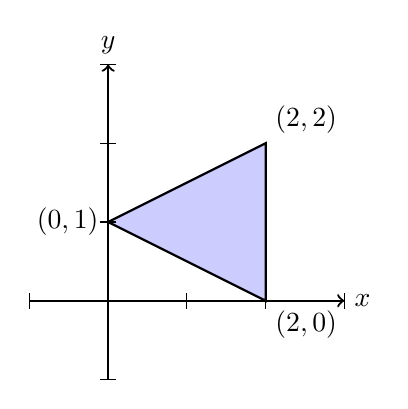
\begin{tikzpicture}[scale=1]
                      % Dibujar los ejes coordenados
                      \draw[->, thick] (-1, 0) -- (3, 0) node[right] {$x$}; % Eje x
                      \draw[->, thick] (0, -1) -- (0, 3) node[above] {$y$}; % Eje y

                      % Dibujar el triángulo
                      \draw[thick, fill=blue!20] (2, 0) -- (2, 2) -- (0, 1) -- cycle;

                      % Etiquetas para los vértices
                      \node at (2, 0) [below right] {$(2, 0)$};
                      \node at (2, 2) [above right] {$(2, 2)$};
                      \node at (0, 1) [left] {$(0, 1)$};

                      % Marcas en los ejes (sin números)
                      \foreach \x in {-1, 0, 1, 2, 3} {
                              \draw (\x, -0.1) -- (\x, 0.1); % Marcas en el eje x
                          }
                      \foreach \y in {-1, 0, 1, 2, 3} {
                              \draw (-0.1, \y) -- (0.1, \y); % Marcas en el eje y
                          }
                  \end{tikzpicture}
              \end{center}
              Intentemos
              calcular $$\int_D x^2y \,dx\,dy = \int_{\mathbb{R}^2} x^2y \cdot \chi_D
                  \,dx\,dy = \int_{x = -\infty}^{x = +\infty} \left(\int_{D_x}x^2\chi_Ddy\right)dx$$
              Sabiendo que $D_x = \{y \in \mathbb{R} : (x,y) \in D\}$, si $0 \leq x \leq 2$
              entonces $D_x = \{y : -\frac{1}{2}x + 1 \leq y \leq \frac{1}{2}x+1\}$\\ Por
              tanto, podemos plantear la integral como: $$= \int_{x = 0}^{x =2} \left(
                  \int_{y = -\frac{1}{2}x + 1}^{y = \frac{1}{2}x + 1} x^2y \,dy \right) dx =
                  \int_{0}^{2}x^2\left(\frac{1}{2} \left(\left(\frac{1}{2}x +1\right)^2-\left(-\frac{1}{2}x+1\right)^2 \right) \right)dx$$
              $$ = \int_{0}^{2}x^2(x) dx = \int_{0}^{2}x^3dx = \frac{16}{4} = 4$$\\ También podríamos haberlo planteado
              así, sabiendo que $D^y = \{x : (x,y) \in D\}$: $$\int_{y =0}^{y =
                      2}\left(\int_{D^y}x^2y \,dx\right)dy = \int_{y = 0}^{y = 1}\left(\int_{x =
                          2(1+y)}^{x =2}x^2y\,dx\right)dy + \int_{y = 1}^{y = 2}\left(\int_{x =
                          2(y-1)}^{x = 2}x^2y\,dx\right)dy.$$ Evaluamos:
              $$\int_{1}^{2}y\left(\int_{2(y-1)}^{2}x^2dx\right)dy =
                  \int_{1}^{2}y\left(\frac{8}{3}y^3 - 4y^2 + 4y\right)dy = \frac{1}{3}y^4 -
                  \frac{4}{3}y^3 + 2y^2 \Big|_{1}^{2} = 4$$

              %2%
        \item Sea $D = \{(x,y) : 0 \leq x \leq y\}$ y $f(x,y) = xe^{-y^3}$. Calculemos:
              $$\int_{D}f(x,y)dxdy.$$ Dado que $f\geq 0$, podemos aplicar el Teorema de
              Tonelli: $$\int_{D}f(x,y)dxdy = \int_{\mathbb{R}^2}f\chi_D = \int_{x = 0}^{x =
                      +\infty}\left(\int_{y = x}^{y = +\infty}e^{-y^3}dy\right)dx$$ No obstante, no
              conocemos el valor de la integral $\int_{y = x}^{y = +\infty}e^{-y^3}dy$, por
              lo que continuamos el cálculo en el otro sentido: $$\int_{y = 0}^{y =
                      +\infty}\left(e^{-y^3}\int_{x = 0}^{x = y}xdx\right)dy = \int_{y = 0}^{y =
                      +\infty}e^{-y^3}\left[\frac{x^2}{2}\right]^{x = y}_{x = 0}dy$$ Evaluamos:
              $$\int_{y = 0}^{y = +\infty}e^{-y^3}\frac{y^2}{2}dy =
                  \left(-\frac{1}{2}\right)\frac{1}{3}\int_{y = 0}^{y = +\infty}e^{-y^3}(-3y^2)dy
                  = -\frac{1}{6}[e^{-y^3}]_{y = 0}^{y = +\infty} = \frac{1}{6}$$

              %3%
        \item Sea $V$ el sólido limitado por $x = 0, \ y = 0, \ z = 0, \ 3x + 2y +z = 1$.
              Calculemos:
              \begin{enumerate}[label=(\alph*)]
                  \item $\text{Vol}(V)$
                  \item $\int_{V}z^2dxdydz$
              \end{enumerate}
              \vspace{-1.5cm}
              \begin{center}
                  \tdplotsetmaincoords{70}{120} % Ángulos para la perspectiva 3D
                  \begin{tikzpicture}[scale=2, tdplot_main_coords]
                      % Definir los ejes
                      \draw[->, thick] (0, 0, 0) -- (1.5, 0, 0) node[right] {$x$};
                      \draw[->, thick] (0, 0, 0) -- (0, 1.5, 0) node[above] {$y$};
                      \draw[->, thick] (0, 0, 0) -- (0, 0, 1.5) node[below left] {$z$};

                      % Definir los puntos de intersección del plano 3x + 2y + z = 1 con los ejes
                      \coordinate (A) at (1/3, 0, 0); % Intersección con el eje x
                      \coordinate (B) at (0, 1/2, 0); % Intersección con el eje y
                      \coordinate (C) at (0, 0, 1);   % Intersección con el eje z

                      % Dibujar el plano 3x + 2y + z = 1
                      \filldraw[fill=blue!20, opacity=0.7] (A) -- (B) -- (C) -- cycle;

                      % Dibujar las aristas del sólido
                      \draw[thick] (A) -- (B) -- (C) -- cycle;
                      \draw[thick] (0, 0, 0) -- (A);
                      \draw[thick] (0, 0, 0) -- (B);
                      \draw[thick] (0, 0, 0) -- (C);

                      % Etiquetas para los puntos de intersección
                      \node at (A) [above left] {$\left(\frac{1}{3}, 0, 0\right)$};
                      \node at (B) [above right] {$\left(0, \frac{1}{2}, 0\right)$};
                      \node at (C) [above left] {$\left(0, 0, 1\right)$};
                  \end{tikzpicture}

              \end{center}
              \begin{itemize}
                  \item[\textbf{(a)}]        Aplicamos el Lema de Cavalieri:
                        $$\text{Vol}(V) = \int_{\mathbb{R}^3} \chi_V(x,y,z)\,dx\,dy\,dz = \int_{z = 0}^{z = 1} \left(\int_{V_z}1dxdy\right)dz,$$
                        donde $V_z = \{(x,y) : (x,y,z) \in V\} = \{(x,y) : x \geq 0, y \geq 0, 3x + 2y \leq 1 - z\}$.

                        Definimos: $$\int_{z = 0}^{z = 1} \text{área}(V_z) dz,$$ donde el área de $V_z$
                        es: $$\text{área}(V_z) = \frac{1}{2} \cdot \frac{1-z}{3} \cdot \frac{1-z}{2}.$$
                        También se podría haber definido como: $$\int_{z = 0}^{z =1}\left(\int_{y =
                                0}^{y = \frac{1-z}{2}}\left(\int_{x = 0}^{x =
                                \frac{1-z-2y}{3}}1dx\right)dy\right)dz.$$ Otra forma alternativa de orden de
                        integración sería: $$\int_{y = 0}^{y = \frac{1}{2}}\left(\int_{z = 0}^{z =
                                    1}\left(\int_{x = 0}^{x = \frac{1-z-2y}{3}}1dx\right)dz\right)dy.$$
                  \item[\textbf{(b)}]  $$\int_{V}z^2dxdydz = \int_{z = 0}^{z = 1}z^2(\int_{V_z}1dxdy)dz = \int_{z = 0}^{z = 1}z^2\cdot\frac{(1-z)^2}{12}dz$$
              \end{itemize}
        \item Sea $V$ el sólido limitado por el paraboloide $z = x^2 +y^2$ y por el plano
              $z=1$.\\ Calculemos $vol(V)$.

              % remove a line
              \vspace{-1cm}
              \begin{center}
    \tdplotsetmaincoords{75}{135}
    \begin{tikzpicture}[tdplot_main_coords,scale=2.0]
        \tikzmath{function f(\x) {return \x;};}
        \pgfmathsetmacro{\zini}{0.5*sqrt(2.0)}
        \pgfmathsetmacro{\step}{0.01}
        \pgfmathsetmacro{\zsig}{\zini+\step}
        \pgfmathsetmacro{\nextz}{\zini+0.5*\step}
        \pgfmathsetmacro{\sig}{2.0*\step}
        \pgfmathsetmacro{\tini}{0.5*pi}
        \pgfmathsetmacro{\tfin}{1.85*pi}
        \pgfmathsetmacro{\tend}{2.5*pi}
        %%% Coordinate axis
        \draw[thick,->] (0,0,0) -- (1.5,0,0) node [below left] {\footnotesize$x$};
        \draw[dashed] (0,0,0) -- (-1.5,0,0);
        \draw[thick,->] (0,0,0) -- (0,1.5,0) node [right] {\footnotesize$y$};
        \draw[dashed] (0,0,0) -- (0,-1.5,0);
        \draw[thick] (0,0,0) -- (0,0,1.0); % Z axis (part under the plane z = 1)
        % The region of integration
        \draw[gray,thick,fill=yellow!20,opacity=0.75] plot[domain=0:6.2832,smooth,variable=\t] ({1.0*cos(\t r)},{1.0*sin(\t r)},{0.0});
        %	
        \draw[gray,dash dot dot] (-1,0,0) -- (-1,0,1);
        \draw[gray,dash dot dot] (0,-1,0) -- (0,-1,1);
        % The plane: x + y = 1
        \coordinate (A) at (1,1,1);
        \coordinate (B) at (-1,1,1);
        \coordinate (C) at (-1,-1,1);
        \coordinate (D) at (1,-1,1);
        % Curves bounding the solid.
        \draw[blue,thick,opacity=0.5] plot[domain=-1:1,smooth,variable=\t] ({\t},0,{\t*\t});
        \draw[blue,thick,opacity=0.5] plot[domain=-1:1,smooth,variable=\t] (0,{\t},{\t*\t});
        \draw[blue,thick,opacity=0.5] plot[domain=0:6.2832,smooth,variable=\t] ({1.0*cos(\t r)},{1.0*sin(\t r)},{1.0});
        % The paraboloid (level curves z = constant)
        \foreach \altura in {\step,\sig,...,1.0}{
                \pgfmathparse{sqrt(\altura)}
                \pgfmathsetmacro{\radio}{\pgfmathresult}
                \draw[blue!20,thick,opacity=0.5] plot[domain=0:6.2832,smooth,variable=\t] ({\radio*cos(\t r)},{\radio*sin(\t r)},{\altura});
            }
        % The plane
        \draw[white] (C) -- (B) node[red,above,sloped,midway]{$z = 1$};
        \fill[pattern color=pink,pattern=north east lines] (A) -- (B) -- (C) -- (D) -- (A);
        \draw[thick,red] (A) -- (B) -- (C) -- (D) -- (A);
        %
        \draw[gray,dash dot dot] (1,0,0) -- (1,0,1);
        \draw[gray,dash dot dot] (0,1,0) -- (0,1,1);
        %
        \node[blue,left] at (0.5,-0.75,0.5) {$z = x^2 + y^2$};
        \draw[thick,->] (0,0,1.0) -- (0,0,1.5) node [above] {\footnotesize$z$};
    \end{tikzpicture}
\end{center}
              \vspace{-2cm}

              Donde $$V = \{(x,y,z) \in \mathbb{R}^3 : x^2 + y^2 \leq z \leq 1\} \implies
                  \\$$ $$vol(v) = \int_{z = 0}^{z = 1}area(V_z)dz = \int_{0}^{1}\pi z dz =
                  \frac{\pi}{2}$$. \\
    \end{enumerate}
}

\begin{observación}
La diferencia entre el Teorema de Tonelli y el de Fubini, es que el primero pide que las funciones sean no-negativas estrictamente y el segundo pide que las funciones sean integrables absolutamente.
\end{observación}
